\documentclass[11pt,a4paper]{article}
\usepackage[utf8]{inputenc}
\usepackage[T1]{fontenc}
\usepackage{lmodern}
\usepackage{geometry}
\usepackage{booktabs}
\usepackage{longtable}
\usepackage{graphicx}
\geometry{margin=2.5cm}
\title{Ocena atrakcyjności inwestycji przy użyciu systemu wnioskowania rozmytego}
\author{Piotr Przymus 127902}
\date{3 maja 2026}
\begin{document}
\maketitle

\section{Wprowadzenie}
Celem pracy było zaprojektowanie systemu wnioskowania rozmytego wspomagającego ocenę
atrakcyjności inwestycji. Model został zaimplementowany z wykorzystaniem biblioteki
jFuzzyLogic oraz standardu FCL (Fuzzy Control Language).

\section{Opis problemu i zmienne}
Ocena atrakcyjności inwestycji polega na określeniu, czy dana inwestycja jest opłacalna,
biorąc pod uwagę możliwy zysk, ryzyko oraz dostępność środków. W praktyce decyzje inwestycyjne
rzadko są jednoznaczne, ponieważ poszczególne czynniki często mają charakter nieprecyzyjny
(np. „wysokie ryzyko” czy „dobra płynność”).

Celem zaprojektowanego systemu jest wspomaganie takiej decyzji poprzez połączenie kilku
kluczowych parametrów w jedną syntetyczną ocenę atrakcyjności. System nie zastępuje
decyzji inwestora, ale stanowi narzędzie pomocnicze, które porządkuje informacje
i ułatwia porównywanie różnych wariantów.

W modelu uwzględniono trzy zmienne wejściowe:
\begin{itemize}
  \item \textbf{Oczekiwana stopa zwrotu} (\textit{expected\_return}) - określa potencjalny zysk z inwestycji;
  \item \textbf{Poziom ryzyka} (\textit{risk}) - opisuje niepewność i możliwość poniesienia strat;
  \item \textbf{Płynność} (\textit{liquidity}) - informuje, jak łatwo można wycofać środki z inwestycji.
\end{itemize}

Zmienne te zostały dobrane tak, aby odzwierciedlały najważniejsze aspekty decyzji inwestycyjnej,
czyli relację między zyskiem a bezpieczeństwem oraz dostępnością kapitału.

Zmienna wyjściowa:
\begin{itemize}
  \item \textbf{Atrakcyjność} (\textit{attractiveness}) - końcowa ocena inwestycji w skali 0--100,
  interpretowana lingwistycznie jako niska, średnia lub wysoka.
\end{itemize}

Zastosowanie logiki rozmytej pozwala na uwzględnienie nieprecyzyjnych pojęć oraz wiedzy eksperckiej
wyrażonej w postaci reguł językowych. Dzięki temu model lepiej odzwierciedla rzeczywisty proces
podejmowania decyzji niż klasyczne podejścia oparte wyłącznie na sztywnych progach liczbowych.

Funkcje przynależności oraz ich parametry zostały zdefiniowane w pliku FCL \texttt{investment.fcl}.

\section{Definicja zmiennych lingwistycznych}

W systemie rozmytym wykorzystano cztery zmienne lingwistyczne: trzy wejściowe i jedną wyjściową.
Każda zmienna została opisana zakresem wartości, zbiorami lingwistycznymi oraz funkcjami przynależności
zdefiniowanymi w pliku FCL.

\subsection{Zmienna \textit{expected\_return}}
\begin{itemize}
  \item zakres: $[0, 30]$,
  \item wartości lingwistyczne: \textit{low}, \textit{medium}, \textit{high},
  \item funkcje przynależności: trapezowe i trójkątne, zdefiniowane w \texttt{investment.fcl}.
\end{itemize}

\subsection{Zmienna \textit{risk}}
\begin{itemize}
  \item zakres: $[0, 10]$,
  \item wartości lingwistyczne: \textit{low}, \textit{medium}, \textit{high},
  \item funkcje przynależności: trapezowe i trójkątne, zdefiniowane w \texttt{investment.fcl}.
\end{itemize}

\subsection{Zmienna \textit{liquidity}}
\begin{itemize}
  \item zakres: $[0, 10]$,
  \item wartości lingwistyczne: \textit{low}, \textit{medium}, \textit{high},
  \item funkcje przynależności: trapezowe i trójkątne, zdefiniowane w \texttt{investment.fcl}.
\end{itemize}

\subsection{Zmienna wyjściowa \textit{attractiveness}}
\begin{itemize}
  \item zakres: $[0, 100]$,
  \item wartości lingwistyczne: \textit{low}, \textit{medium}, \textit{high},
  \item funkcje przynależności: trapezowe i trójkątne, zdefiniowane w \texttt{investment.fcl}.
\end{itemize}

Tak zdefiniowane zmienne pozwalają przełożyć jakościowe oceny inwestycji na model rozmyty,
w którym reguły eksperckie mogą łączyć informację o potencjalnym zysku, ryzyku i płynności w jedną
syntetyczną ocenę atrakcyjności.

Formalnie każda zmienna lingwistyczna została zdefiniowana jako piątka
$L = (X, T(X), U, G, M)$, gdzie $X$ oznacza nazwę zmiennej, $T(X)$ zbiór wartości
lingwistycznych, $U$ uniwersum rozważań, $G$ reguły generowania nazw, natomiast $M$
odwzorowanie przypisujące funkcje przynależności.

\section{Baza reguł}
Zdefiniowano 11 reguł rozmytych. Jest to model uproszczony, czyli nie obejmuje wszystkich możliwych
kombinacji trzech wartości lingwistycznych dla trzech zmiennych (takich kombinacji byłoby 27), lecz
tylko najistotniejsze i najbardziej reprezentatywne przypadki decyzyjne. Dzięki temu model jest
czytelniejszy, łatwiejszy do interpretacji i prostszy w utrzymaniu.

Reguły sformułowano zgodnie z intuicją dotyczącą relacji między zmiennymi: niska stopa zwrotu
połączona z wysokim ryzykiem lub niską płynnością obniża atrakcyjność, a odwrotne warunki ją podwyższają.
Reguły pośrednie (np. mieszanka średnich i wysokich wartości wejść) pozwalają uzyskać wartości pośrednie
wyjściowe.

Pełna baza reguł:
\begin{longtable}{ll}
\toprule
Nr & Reguła \\
\midrule
1 & IF expected\_return IS low AND risk IS high THEN attractiveness IS low \\
2 & IF expected\_return IS low AND liquidity IS low THEN attractiveness IS low \\
3 & IF expected\_return IS medium AND risk IS medium AND liquidity IS medium THEN attractiveness IS medium \\
4 & IF expected\_return IS high AND risk IS low AND liquidity IS high THEN attractiveness IS high \\
5 & IF expected\_return IS high AND risk IS medium THEN attractiveness IS medium \\
6 & IF expected\_return IS medium AND risk IS low THEN attractiveness IS high \\
7 & IF expected\_return IS high AND liquidity IS low THEN attractiveness IS medium \\
8 & IF risk IS high AND liquidity IS low THEN attractiveness IS low \\
9 & IF expected\_return IS low AND risk IS low AND liquidity IS high THEN attractiveness IS medium \\
10 & IF expected\_return IS medium AND liquidity IS high THEN attractiveness IS high \\
11 & IF expected\_return IS high AND risk IS high THEN attractiveness IS medium \\
\bottomrule
\end{longtable}

Z punktu widzenia interpretacji eksperckiej reguły 1--2 odzwierciedlają sytuacje niekorzystne,
reguły 4, 6 i 10 opisują warunki atrakcyjne, a reguły 3, 5, 7, 8, 9, 11 stanowią przypadki pośrednie.


\section{Metoda defuzyfikacji}
Zastosowano metodę środka ciężkości (COG) - jest ona jedną z najczęściej
wykorzystywanych metod defuzyfikacji w systemach rozmytych.

W implementacji w jFuzzyLogic metoda jest ustawiona w sekcji DEFUZZIFY zmiennej wyjściowej:
\begin{verbatim}
METHOD : COG;
DEFAULT := 0;
\end{verbatim}

\section{Eksperymenty i wyniki}
Dla modelu uproszczonego dobrano 11 reprezentatywnych przypadków testowych, po jednym dla kluczowych
reguł oraz przypadków brzegowych. Dla każdego terminu lingwistycznego przyjęto reprezentatywne
wartości numeryczne (centra funkcji przynależności):
\begin{itemize}
  \item `expected\_return`: low=3.0, medium=10.0, high=20.0,
  \item `risk`: low=1.0, medium=5.0, high=10.0,
  \item `liquidity`: low=2.0, medium=5.0, high=8.0.
\end{itemize}
Wyniki eksperymentów zostały zarejestrowane w postaci danych liczbowych,
obejmujących wartości zmiennych wejściowych oraz odpowiadające im wartości
zmiennej wyjściowej.

\subsection{Wyniki numeryczne}
Analizę przeprowadzono na 11 przypadkach odpowiadających wybranym, najbardziej reprezentatywnym
kombinacjom wejść. Podstawowe statystyki atrakcyjności to:
\begin{itemize}
  \item liczba przypadków: 11,
  \item wartość minimalna: 0.00,
  \item wartość maksymalna: 80.53,
  \item wartość średnia: około 50.02.
\end{itemize}

Rozkład wyników wykazuje skupienia w trzech typowych poziomach: wartości niskie (około 0--20),
wartości średnie (około 50) oraz wysokie (około 80). To zachowanie jest konsekwencją zastosowanych
funkcji przynależności, operatorów logicznych (AND=MIN) oraz metody akumulacji (MAX) i defuzyfikacji
(COG). W praktyce oznacza to, że model rozpoznaje zarówno sytuacje niekorzystne, neutralne, jak i
wyraźnie atrakcyjne.

Interpretacja lingwistyczna wyników została wykonana na podstawie dominującego
stopnia przynależności do zbiorów rozmytych. Wartości pośrednie mogą należeć do
więcej niż jednego zbioru, jednak przypisywane są do tego, dla którego stopień
przynależności jest największy.

\subsection{Tabela (opisowa)}
W tabeli poniżej przedstawiono 11 przypadków testowych w formie opisowej.
% Ta tabela została wygenerowana automatycznie przez generate_results_table.py
\begin{table}[h]
\centering
\caption{Wyniki (opisowo) dla modelu uproszczonego}
\label{tab:results_desc}
\begin{tabular}{ccccc}
\toprule
Lp. & Stopa zwrotu & Ryzyko & Płynność & Atrakcyjność \\ 
\midrule
1 & niska & wysoki & niska & niska \\ 
2 & niska & niski & niska & niska \\ 
3 & średnia & średni & średnia & średnia \\ 
4 & wysoka & niski & wysoka & wysoka \\ 
5 & wysoka & średni & średnia & średnia \\ 
6 & średnia & niski & średnia & wysoka \\ 
7 & wysoka & wysoki & niska & niska \\ 
8 & średnia & wysoki & niska & niska \\ 
9 & niska & niski & wysoka & średnia \\ 
10 & średnia & średni & wysoka & wysoka \\ 
11 & wysoka & wysoki & średnia & średnia \\ 
\bottomrule
\end{tabular}
\end{table}


\section{Analiza i wnioski}
Uzyskane wyniki pokazują, że model działa zgodnie z przyjętymi założeniami.

\begin{itemize}
  \item niska stopa zwrotu połączona z wysokim ryzykiem i niską płynnością prowadzi do niskiej atrakcyjności inwestycji,
  \item wysoka stopa zwrotu przy niskim ryzyku i wysokiej płynności daje wysoką ocenę atrakcyjności,
  \item przypadki pośrednie generują wyniki średnie, zależne od aktywowanych reguł.
\end{itemize}

Można zauważyć, że system poprawnie rozróżnia inwestycje niekorzystne, neutralne oraz atrakcyjne.
Najwyższe wartości pojawiają się dla inwestycji o korzystnym stosunku zysku do ryzyka, natomiast
najniższe dla konfiguracji o dużym ryzyku i słabych pozostałych parametrach.

Wyniki około 50 odpowiadają przypadkom mieszanym, w których część parametrów jest korzystna,
a część nie. Pokazuje to, że system nie podejmuje decyzji w sposób zero-jedynkowy, lecz uwzględnia
stopień spełnienia poszczególnych warunków.

Zaprojektowany model jest prosty, czytelny i łatwy do interpretacji. Daje wyniki zgodne z intuicją i pozwala w prosty sposób porównywać różne warianty inwestycji. Można go rozszerzyć o większą liczbę reguł lub dostrojenie funkcji przynależności na podstawie danych
historycznych.

\section{Wizualizacja funkcji przynależności}
Poniżej przedstawiono wykresy funkcji przynależności dla wszystkich zmiennych
wykorzystanych w modelu - łatwo zauważyć zakresy aktywacji.

\begin{figure}[ht]
  \centering
  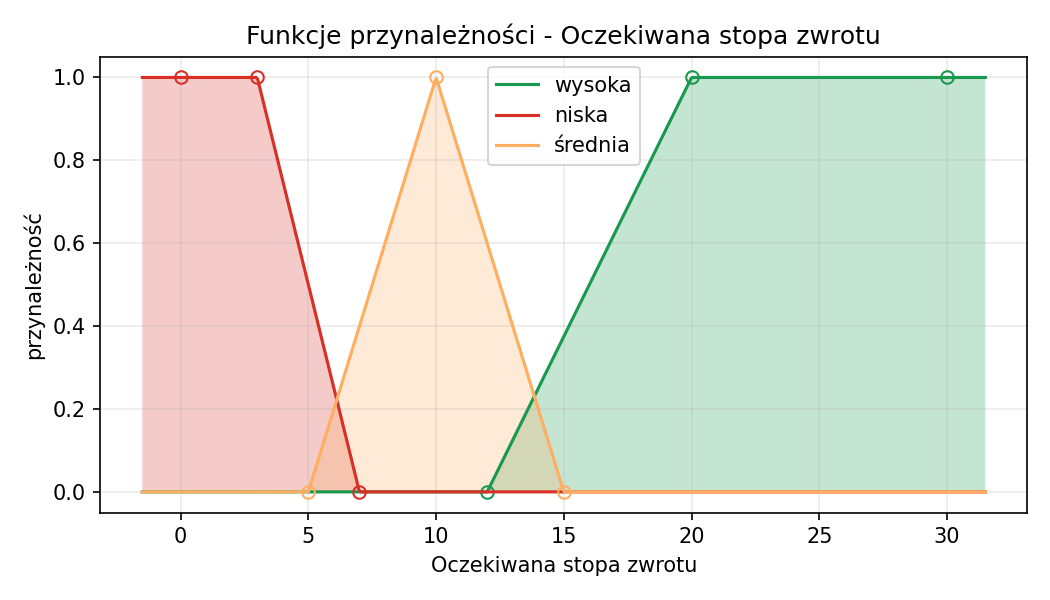
\includegraphics[width=0.8\textwidth]{plots/expected_return.png}
  \caption{Funkcje przynależności dla zmiennej wejściowej: oczekiwana stopa zwrotu}
  \label{fig:mf_expected_return}
\end{figure}

\begin{figure}[ht]
  \centering
  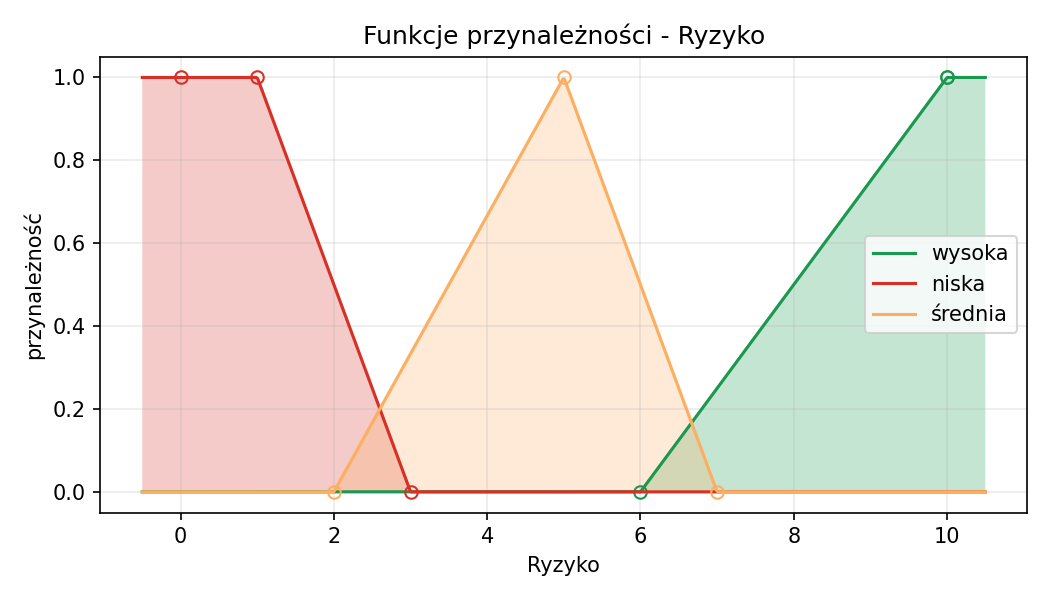
\includegraphics[width=0.8\textwidth]{plots/risk.png}
  \caption{Funkcje przynależności dla zmiennej wejściowej: ryzyko}
  \label{fig:mf_risk}
\end{figure}

\begin{figure}[ht]
  \centering
  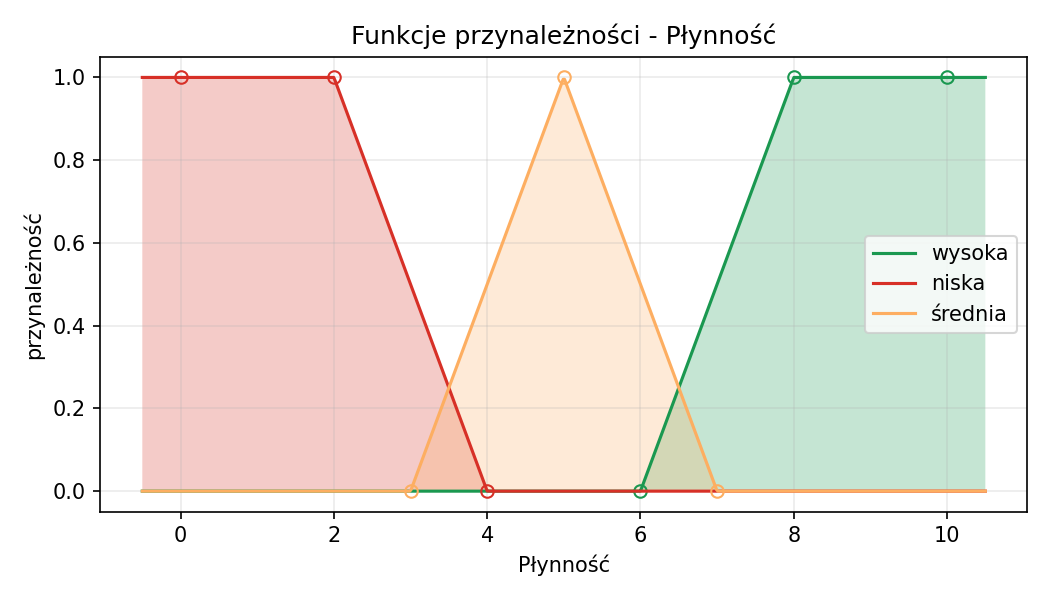
\includegraphics[width=0.8\textwidth]{plots/liquidity.png}
  \caption{Funkcje przynależności dla zmiennej wejściowej: płynność}
  \label{fig:mf_liquidity}
\end{figure}

\begin{figure}[ht]
  \centering
  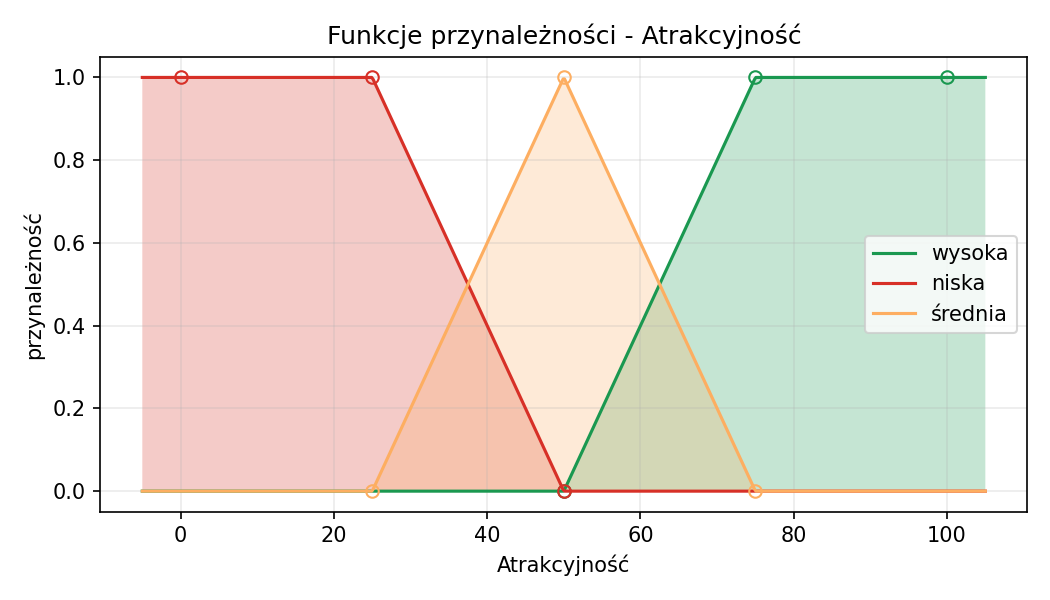
\includegraphics[width=0.8\textwidth]{plots/attractiveness.png}
  \caption{Funkcje przynależności dla zmiennej wyjściowej: atrakcyjność}
  \label{fig:mf_attractiveness}
\end{figure}

\end{document}
